\documentclass[a4paper,12pt,exos]{nsi} 
\usepackage{mathtools}
\usepackage{hyperref}



\pagestyle{empty}

\begin{document}
    \classe{\premiere spe}
    \titre{Modéliser avec des fonctions}
    \maketitle

    \begin{minipage}{12cm}
        Pour préparer la saison touristique à Martin-Plage, la mairie souhaite délimiter une aire de baignade rectangulaire.\\
        Elle dispose d'un kit pour délimiter la zone de baignade.
    \end{minipage}
    \begin{minipage}{5cm}
        \flushright 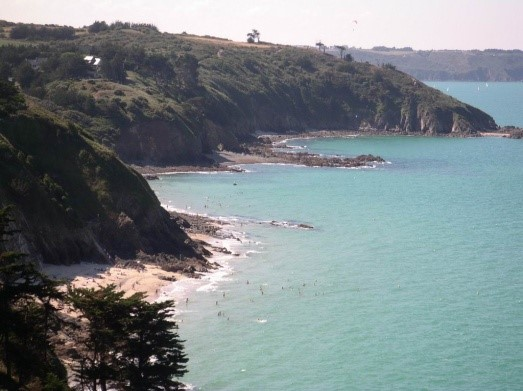
\includegraphics[width=4cm]{martinplage}\\
        \small Martin-Plage, Plérin
    \end{minipage}
    
    \begin{encadrecolore}{Document 1 :}{UGLiBlue}
        \textbf{Kit pour la confection d'une zone de baignade}\\
        
        \begin{minipage}{8cm}
            Offre « package » pour monter une ligne d'eau de balisage de bain de 90 m comprenant le cordage (diamètre 20 mm) et les flotteurs rouges.
        \end{minipage}
        \begin{minipage}{8cm}
            \flushright 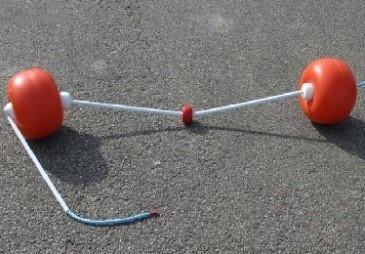
\includegraphics[height=2.6cm]{flotteurs} \hspace{.2cm} 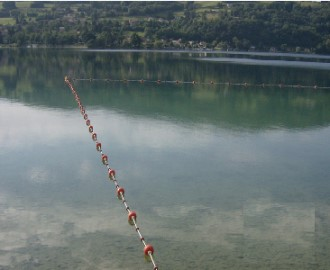
\includegraphics[height=2.6cm]{flotteurs2}
        \end{minipage}
    \end{encadrecolore}
    
    \begin{encadrecolore}{Document 2 :}{UGLiBlue}
        \textbf{Normes d’hygiène et de sécurité applicables aux baignades aménagées}\\
        
        La fréquentation maximale instantanée en baigneurs présents dans l’établissement ne doit pas dépasser trois personnes pour 2 mètres carrés de plan d’eau en plein air et une personne par mètre carré de plan d’eau couvert. Pour l’application du présent article, la surface des pataugeoires et celle des bassins de plongeon ou de plongée réservés en permanence à cet usage ne sont pas prises en compte dans le calcul de la surface des plans d’eau.\\[.5em]
        \textit{Légifrance- Article D 1332 – 10 Modifié par Décret n°2006-676 du 8 juin 2006 – art.2 JORF 10 Juin 2006}
    \end{encadrecolore}
    
    \textbf{Combien de baigneurs pourra-t-on accueillir au maximum dans la zone de baignade ?}\\
    
    \dleft{13.5cm}{
        Présenter à l’oral durant 2 minutes maximum la situation, la solution, les outils de modélisation et les moyens d’y accéder.\\

        \textit{Lien pour l'enregistrement :} \href{https://www.mon-oral.net/a/MZE4MG9V}{https://www.mon-oral.net/a/MZE4MG9V}
    }
    {
\includegraphics[width=3cm]{code-qr.png}}
    
    \newpage
    \textbf{Grille d'évaluation :} \textit{(d'après la grille d'évaluation
        indicative du Grand Oral)
    }
    \begin{enumerate}[label=\textbullet]
        \item 	\textbf{Qualité de la parole :} qualité orale de la prestation\\[.5em]
        \begin{tabular}{|p{3.8cm}|p{3.8cm}|p{3.8cm}|p{3.8cm}|}
            \hline
            Insuffisant & Fragile & Satisfaisant & Très satisfaisant\\
            \hline
            Difficilement audible sur l'ensemble de la prestation.\newline
            Ne parvient pas à capter l'attention. &
            La voix devient plus audible et intelligible au fil de la prestation mais demeure monocorde.\newline
            Vocabulaire limité ou approximatif &
            Quelques variations dans l'utilisation de la voix ; prise de parole affirmée.\newline
            Le candidat parvient à susciter l'intérêt.\newline
            Utilisation d'un vocabulaire adapté.&
            La voix soutient efficacement le discours.\newline
            Débit du discours adapté, fluidité, variations et nuances pertinentes.\newline
            Le candidat est pleinement engagé dans sa parole.\newline
            Utilisation d'un vocabulaire riche et précis.
    \\
            \hline
        \end{tabular}
        \vspace{.5cm}
        
        \item 	\textbf{Qualité du discours :} qualité de la prise de parole en continu\\[.5em]
        \begin{tabular}{|p{3.8cm}|p{3.8cm}|p{3.8cm}|p{3.8cm}|}
            \hline
            Insuffisant & Fragile & Satisfaisant & Très satisfaisant\\
            \hline
            Énoncés courts, ponctués de pauses et de faux démarrages ou énoncés longs à la syntaxe mal maîtrisée. &
            Discours assez clair mais vocabulaire limité et énoncés approximatifs.  &
            Discours bien organisé ; énoncés bien construits.&
            Discours fluide, efficace, tirant pleinement profit du temps.\newline
            Les choix effectués dans la présentation sont pertinents.
    \\
            \hline
        \end{tabular}
        \vspace{.5cm}
        
        \item 	\textbf{Qualité des connaissances :}\\[.5em]
        \begin{tabular}{|p{3.8cm}|p{3.8cm}|p{3.8cm}|p{3.8cm}|}
            \hline
            Insuffisant & Fragile & Satisfaisant & Très satisfaisant\\
            \hline
            Connaissances imprécises, incapacité à répondre au problème. &
            Connaissances réelles, mais difficultés à les mobiliser dans la situation proposée.  &
            Connaissances précises, une capacité à les mobiliser.\newline
            Quelques manques dans la rigueur du raisonnement.
     &
            Connaissances maîtrisées, recherche de rigueur dans les justifications.
    
    \\
            \hline
        \end{tabular}
    \end{enumerate}

\end{document}